\chapter{Estado del arte}
En esta sección se van a presentar algunos de los hipervisores más populares utilizados en sistemas embebidos y sus características principales, poniendo más énfasis en los casos de Xen y Jailhouse ya que se tratan de los hipervisores que se han utilizado para el desarrolo del actual TFM. Estos dos últimos resultan de mayor interés debido a que son de código abierto, por lo que aparte de la documentación oficial, a veces un poco escasa en los proyectos de código abierto, exiten repositorios públicos con el código fuente. De esta forma se puede analizar de mejor manera su estructura e incluso modificar partes de su código para adaptarlo a las necesidades del sistema.

\section{OKL4 Hypervisor}
OKL4 Hypervisor es un hipervisor de tipo 1 de los basados en micro-kernel. Fue desarrollado originalmente por OK Labs, la cual forma parte del conglomerado General Dynamics, aprovechando la experiencia en micro-kernels que habían desarrollado gracias al éxito comercial de otro de los productos de OK Labs, el micro-kernel seL4 \cite{seL4}. En su visión, no existían razones para no poder combinar en una única implementación un micro-kernel y un hipervisor. De echo, durante mucho tiempo, el OKL4 se denominó \textit{OKL4 Microvisor}.\\
El objetivo es dar soporte para la virtualización con la mínima sobrecarga del sistema. De esa forma, el modelo propuesto se basa en los siguientes principios \cite{okl4}:
\begin{itemize}
  \item La abstracción de ejecución que presenta el hipervisor a los sistemas operativos guest consta de una o varias CPUs virtuales (vCPU), en las que poder desplegar las tareas requeridas por las aplicaciones de usuario.
  \item En el apartado de virtualización de memoria, el hipervisor proporcioa una MMU virtual (vMMU) con la que se mapea la memoria virtual de los sistemas guest en memoria física del sistema host.
  \item La virtualización de los periféricos, se basa en el mapeo en memoria de registro de dispositivos virtuales y un sistema de interrupciones virtuales (vIRQ).
  \item La comunicacion entre sistemas guest, se muestra como vIRQs (para sincronización) y canales. Los canales se implementan con FIFOs bidireccionales con una tamaño fijo especificado en el espacio de usuario.
\end{itemize}
\begin{figure*}[!htb]
	\centering
	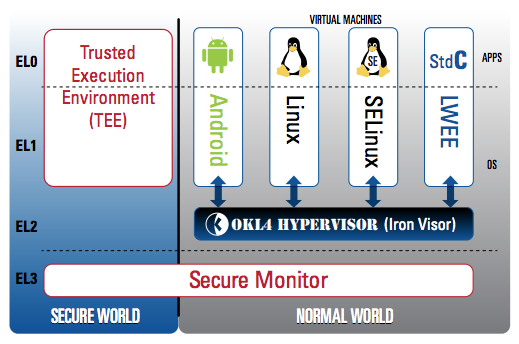
\includegraphics[width=0.65\textwidth]{recursos/OK_L4_Microvisor.png}
	\caption{Ejemplo de arquitectura basada en OKL4 Hypervisor}
	\label{fig:OK_L4_Microvisor}
\end{figure*}
OKL4 Hypervisor proporciona además de soporte de sistemas operativos guest como Linux, VxWorks y Android, un entorno denominado \textit{Lightweight Execution Environments}, que viene a ser un entorno que ofrece rendimentos cercanos a aplicaciones baremetal.\\
Este hipervisor tiene como uno de sus objetivos principales la seguridad \cite{okl4_2} y se hace mucho énfasis en la confiabilidad que proporciona su sitema frente a ataques externos debido al aislamiento proporcionado entre celdas. También destaca su manejo de los recursos para tener la mínima huella de consumo de energía, haciéndolo apto para sistemas que funcionan con batería.


\section{WindRiver Hypervisor}
El hipervisor de WindRiver es también un hipervisor de tipo 1 que particiona el software que se ejecuta en uno o varios núcleos en múltiples tarjetas virtuales (Virtual Boards) con diferentes niveles de protección ya características. Está optimizado para ejecutar sistemas opetativos guest de propósito general (GPOS), sistema de tiempo real y sistemas operativos para aplicaciones críticas de seguridad \cite{windriver_1}.
\subsection{Virtual Boards}
La división del sistema propuesta por WindRiver se basa en tarjetas virtuales o particiones. Cada una de ellas puede contener un sistema operativo guest con sus diferentes aplicaciones ejecutandose o un programa si sistema operativo, lo que se denomina \textit{virtual board application}. El hipervisor es el encargado de controlar en qué núcleos se están ejecutando las virtual boards y las zonas de memoria a las que puede acceder. Una virtual board puede compartir un núcleo con con otra virtual board, tener un núcleo dedicado, o utilizar varios al mismo tiempo.
\begin{figure*}[!htb]
	\centering
	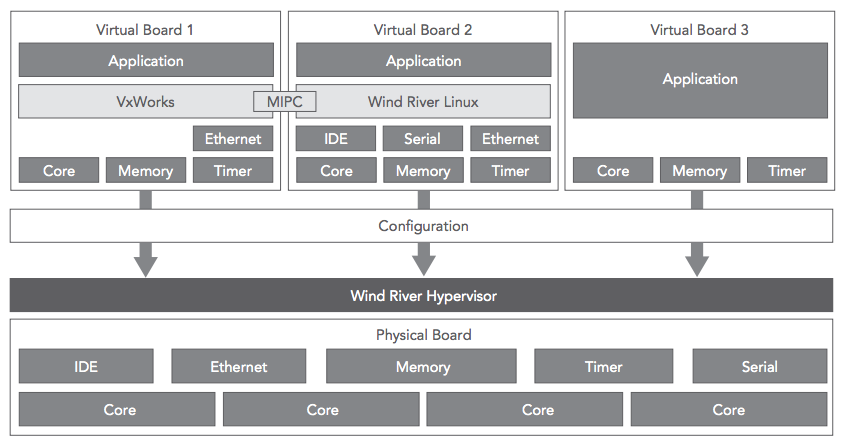
\includegraphics[width=0.75\textwidth]{recursos/windriver_hyp.png}
	\caption{WindRiver Hypervisor}
	\label{fig:windriver_hyp}
\end{figure*}

Las virtual boards pueden ser creadas, arrancadas, detenidas y relanzadas individualemnte. Esto porporciona la opción de escalar dinámicamente la aplicación en función de la demanda en cada momento.

\subsection{Sistemas operativos guest}
El hipervisor de WindRiver es capaz de ejecutar sistemas operativos utilizando una mezcla de virtualización asistida por hardware y paravirtualización con el objetivo de proporcionar un rendimiento óptimo. Soporta sitemas operativos guest como VxWorks o WindRiver Linux, y proporciona una interfaz para que otros sitemas operativos puedan ejecutarse, incluyendo sistemas operativos de código abierto o propietarios.\\

\paragraph{Sistemas operativos sin modificaciones} El hipervisor de WindRiver permite la ejecución de sistemas operativos sin modificaciones de código del tipo Red Hat Enterprise Linux o Microsoft Windows dentro de una virtual board en microprocesadores Intel con extensiones de virtualización.\\

\paragraph{Sistemas baremetal}
El hipervisor permite la ejecución de virtual boards que no tengan sistema operativo denominadas \textit{bare metal executives}. Hay ciertas tareas en los sistemas embebidos que no requieren de capacidades que ofrece un sistema operativo ni la complejidad que añade. WindRiver proporciona una API abierta con la que presenta a estas virtual boards la forma de acceder a los recursos del sistema como la MMU, excepciones e interrupciones, núcleos de CPU y otros dispositivos necesarios para operar. Esta API permite beneficiarse de las capacidades de la virtualización mientras se mantiene la respuesta en tiempo real necesaria por la aplicación.

\paragraph{Paravirtualización y virtualización asistida por hardware}
Como se ha mencionado anteriormente, muchas familias actuales de microprocesadores proporcionan mecanismos hardware para asistir en la virtualización. El hipervisor de WindRiver se vale de estos mecanismos para proporcionar servicios de virtualización. De la misma manera, existen muchos dispositivos que no proporcionan esta asistencia por hardware, y esos servicios de virtualización están implementandos en software impactando en el rendimiento del sistema. Para esos casos se requiere de paravirtualización del sistema operativo.\\
La paravirtualización es la modificación de las llamadas privilegiadas de un sistema operativo para que colabore con el hipervisor. Es este el que debe ejecutar las llamadas privilegiadas en representación del sistema operativo guest. La cantidad de modificaciones necesaria depende mucho de la arquitectura del microprocesador y típicamente implica lo siguiente:

\begin{itemize}
  \item Niveles privilegiados: un sistema virtualizado requiere normalmente de tres niveles de privilegio distintos: uno para el hipervisor, otro para el sistema operativo guest y otro para las aplicaciones. Las arquitecturas de microprocesadores que no proporcionan aistencia por hardware suelen tener solo dos niveles de privilegio. La tarea de la paravirtualización es emular el nivel que falta. Las instrucciones privilegiadas tienen que ser sustituidas por llamadas a la API del hipervisor.
  \item Acceso a dispositivos: un driver en un sistema operativo que se ejecuta nativamente puede acceder a cualquier dispositivo. En un entorno virtualizado, el hipervisor es el que arbitra y decide si una determinada virtual board tiene acceso a un dispositivo o no. Esto incluye interrupciones, dispositivos de entrada salida, registros, y acceso directo a memoria (DMA)
  \item MMU: el hipervisor controla la MMU en un entorno virtualizado. Algunos procesadores con asistencia hardware perimiten a un sistema guest modificar la MMU de la virtual board. Si no se dispone de la asistencia hardware, el guest debe colaborar con el hipervisor para modificar la MMU.
\end{itemize}

\paragraph{Acceso a dispositivos}
El hipervisor de WindRiver proporciona un modelado de dispositivo que permite asignar dispositivos a las virtual boards de diferentes maneras. El acceso al dispositivo puede ser directo, compartido, virtualizado o emulado. Cada una de estas formas de acceder tiene sus particularidades y la elección depende en gran medida de la aplicación y del rendimiento necesario.

\begin{itemize}
  \item Directo: en este modo, el dispositivo es mapeado directamente al espacio de memoria del sistema guest, teniendo este el control exclusivo sobre el dispositivo y no utilizando ninguna característica de la virtualización. El resto de sistemas guest no detectan la existencia del dispositivo. Este modo proporciona el mayor rendimiento posible de acceso.

  \item Compartido: El acceso compartido es deseable cuando un sistema guest de alguna forma posee el acceso al dispositivo (configuración por ejemplo) pero otro sistema guest está interesado en los datos que se producen en dicho dispositivo.
  \begin{figure*}[!htb]
  	\centering
  	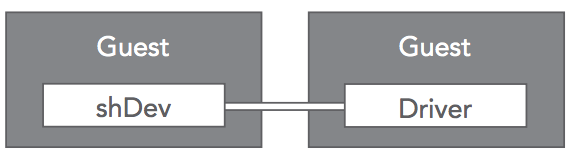
\includegraphics[width=0.65\textwidth]{recursos/windriver_drv_1.png}
  	\caption{acceso compartido a dispositivo en WindRiver Hypervisor}
  	\label{fig:windriver_drv_1}
  \end{figure*}

  \item Virtualizado: este tipo de acceso se utiliza cuando más de un sistema guest requiere de acceso a un dispositivo. De esta forma, el driver propiamente dicho se encuentra dentro del hipervisor y los sitemas guest utilizan un driver ``stub'' para comunicarse con él.
  \begin{figure*}[!htb]
  	\centering
  	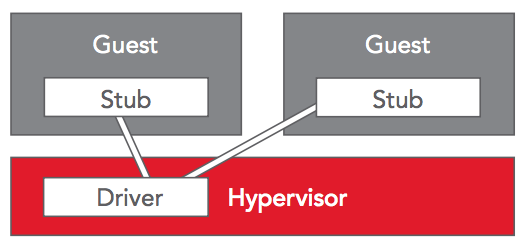
\includegraphics[width=0.65\textwidth]{recursos/windriver_drv_2.png}
  	\caption{acceso virtualizado a dispositivo en WindRiver Hypervisor}
  	\label{fig:windriver_drv_2}
  \end{figure*}

  \item Emulado: el caso de uso para este tipo de acceso a dispositivo es en el que los drivers de los sistemas guest no pueden ser sustituidos por un driver ``stub''. El hipervisor proporciona una emulación hardware al driver nativo del sistema guest pero por debajo utiliza su propio driver para accedes físicamente al dispositivo. Los dispositivos emulados ofrecen la mayor de las flexibilidades para las virtual boards pero el impacto en el rendimiento es significativamente mayor que en el resto de los casos.
  \begin{figure*}[!htb]
  	\centering
  	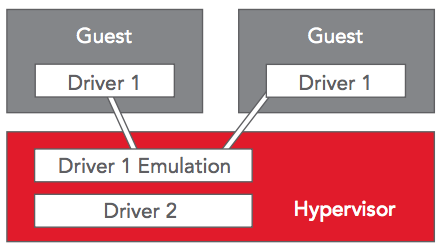
\includegraphics[width=0.65\textwidth]{recursos/windriver_drv_3.png}
  	\caption{acceso emulado a dispositivo en WindRiver Hypervisor}
  	\label{fig:windriver_drv_3}
  \end{figure*}

\end{itemize}

\paragraph{Comunicaciones entre guests}
El hipervisor de WindRiver facilita la comunicación rápida entre virtual boards proporcionando mensajería punto a punto, comunicación entre procesos multi sistema operativo o \textit{multi-OS inter-process communication (MIPC)} (MIPC), y comunicaciones IP usando un controlador virtual de red (VNIC). Existen dos formas de transporte de mensajes: memoria compartida para conexiones MIPC y sistema seguro de transporte tanto para conexiones MIPC como para conexiones VNIC. Las conexiones rápidas por IP entre virtual boards se consiguen utilizando el driver VNIC del sistema guest y creando uno o más switches ethernet virtuales dentro del hipervisor.
\begin{figure*}[!htb]
  \centering
  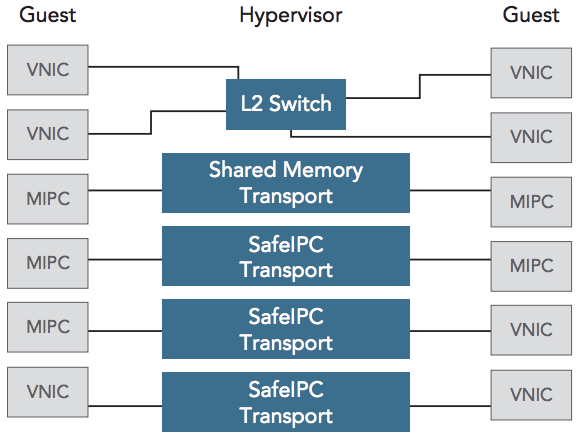
\includegraphics[width=0.65\textwidth]{recursos/windriver_com.png}
  \caption{opciones de comunicación entre virtual boards en WindRiver Hypervisor}
  \label{fig:windriver_com}
\end{figure*}
